\documentclass[border=5pt]{standalone}
% Shared by every figure. Colour marks the TYPE of a quantity, never decoration:
%   blue   (vec) equivariant: rotates with its fragment     -- solid arrows
%   orange (inv) invariant: unchanged by any rotation        -- dashed arrows
%   aqua   (att) attention / communication between elements
%   violet (out) what the network outputs
% Text is always ink; a coloured mark next to it carries the meaning.
\usepackage{amsmath,amssymb,bm}
\usepackage{tikz}
\usetikzlibrary{arrows.meta,positioning,fit,backgrounds,calc,shapes.geometric,
  shapes.misc,decorations.pathreplacing,decorations.pathmorphing,matrix,
  patterns,cd,shadows}
\definecolor{vec}{HTML}{2A78D6}
\definecolor{inv}{HTML}{EB6834}
\definecolor{att}{HTML}{1BAF7A}
\definecolor{out}{HTML}{4A3AA7}
\definecolor{ink}{HTML}{0B0B0B}
\definecolor{ink2}{HTML}{52514E}
\definecolor{ink3}{HTML}{8A877F}
\definecolor{neutral}{HTML}{F0EFEC}
\definecolor{rule}{HTML}{CFCCC4}
\definecolor{pieceA}{HTML}{E4E1DA}
\definecolor{pieceB}{HTML}{CDC9BF}
\definecolor{pieceC}{HTML}{B3AEA2}
\colorlet{vecfill}{vec!9}
\colorlet{invfill}{inv!10}
\colorlet{attfill}{att!11}
\colorlet{outfill}{out!9}
\tikzset{
  >={Stealth[length=2.3mm,width=1.7mm]},
  every picture/.style={line cap=round, line join=round},
  box/.style={draw=ink2, fill=neutral, rounded corners=2.5pt, align=center,
    font=\small, inner sep=4pt, minimum height=8mm, text=ink, line width=0.6pt, nohyph},
  vecbox/.style={box, draw=vec, fill=vecfill},
  invbox/.style={box, draw=inv, fill=invfill},
  attbox/.style={box, draw=att, fill=attfill},
  outbox/.style={box, draw=out, fill=outfill},
  plain/.style={box, draw=ink3, fill=white},
  arr/.style={->, draw=ink2, line width=0.7pt},
  vecarr/.style={->, draw=vec, line width=1.1pt},
  invarr/.style={->, draw=inv, line width=1.1pt, dash pattern=on 3.2pt off 1.8pt},
  attarr/.style={->, draw=att, line width=1.1pt, dash pattern=on 1.2pt off 1.4pt},
  outarr/.style={->, draw=out, line width=1.1pt},
  nohyph/.style={execute at begin node={\hyphenpenalty=10000\exhyphenpenalty=10000\relax}},
  lbl/.style={font=\footnotesize, text=ink2, align=center, nohyph},
  tlbl/.style={font=\footnotesize, text=ink, align=center, nohyph},
  group/.style={draw=ink3, dashed, rounded corners=5pt, inner sep=7pt},
  op/.style={circle, draw=ink2, fill=white, inner sep=0pt, minimum size=5.2mm,
    font=\small, line width=0.6pt},
  piece/.style={fill=#1, draw=none},
  intact/.style={draw=ink2, line width=0.6pt},
  fracture/.style={draw=ink, line width=1.5pt},
  token/.style={circle, fill=att, draw=white, line width=0.5pt, inner sep=0pt,
    minimum size=4.2pt},
  vtx/.style={circle, fill=ink, inner sep=0pt, minimum size=3pt},
  panel/.style={font=\small\bfseries, text=ink, anchor=north west},
}
% one piece of the cartoon, in its own centred frame: fill, intact edge, fracture edge
\newcommand{\drawpiece}[2]{% #1 = A|B|C, #2 = fill colour
  \fill[#2] \csname Piece#1\endcsname;
  \draw[intact] \csname Intact#1\endcsname;
  \draw[fracture] \csname Crack#1\endcsname;}
% a legend entry: a short line in a given style, then its text
\newcommand{\legendline}[3]{% #1 position, #2 style, #3 text
  \draw[#2] (#1) -- ++(0.7,0) node[right, tlbl, text=ink] {#3};}

\begin{document}
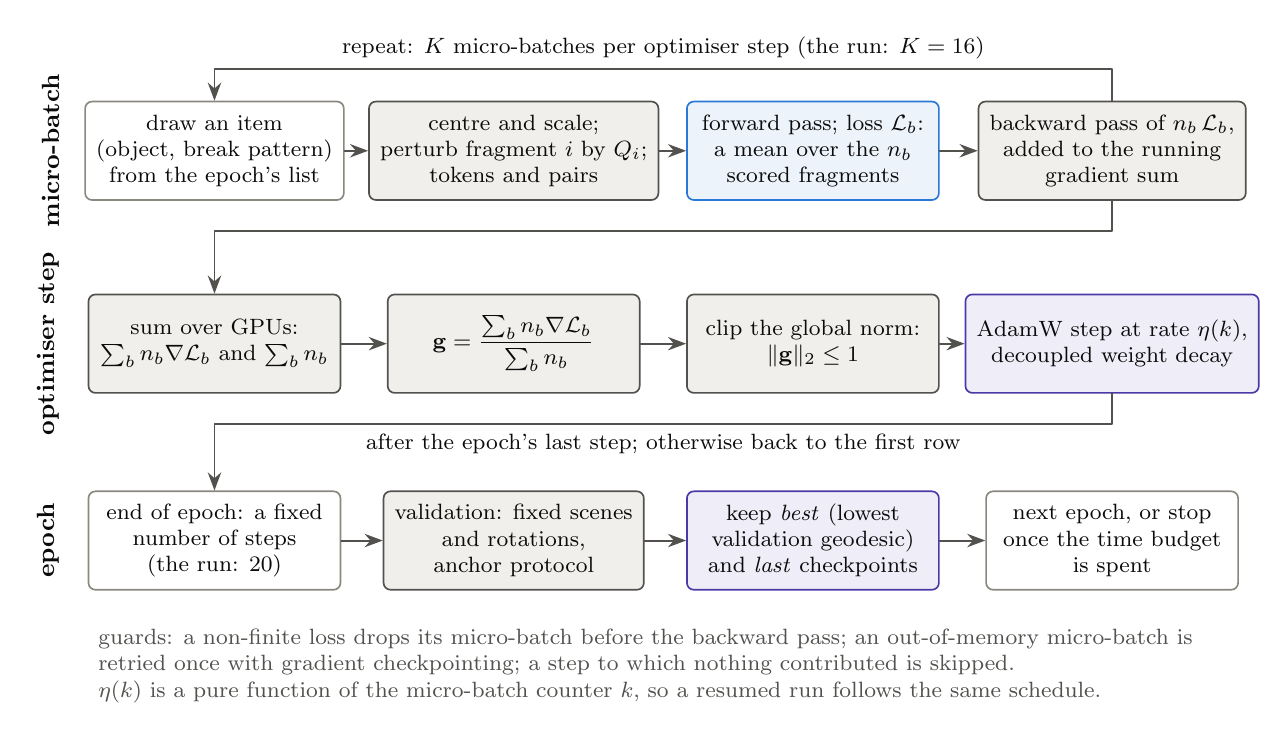
\begin{tikzpicture}
  \tikzset{
    st/.style={box, font=\footnotesize, minimum height=12.5mm, minimum width=3.2cm},
    vst/.style={st, draw=vec, fill=vecfill},
    ost/.style={st, draw=out, fill=outfill},
    pst/.style={st, draw=ink3, fill=white},
    rowlab/.style={font=\small\bfseries, text=ink, rotate=90, anchor=south},
  }
  % ---------------- one micro-batch ----------------
  \node[rowlab] at (-1.85,0) {micro-batch};
  \node[pst] (s1) at (0,0) {draw an item\\ (object, break pattern)\\ from the epoch's list};
  \node[st] (s2) at (3.8,0) {centre and scale;\\ perturb fragment $i$ by $Q_i$;\\ tokens and pairs};
  \node[vst] (s3) at (7.6,0) {forward pass; loss $\mathcal L_b$:\\ a mean over the $n_b$\\ scored fragments};
  \node[st] (s4) at (11.4,0) {backward pass of $n_b\,\mathcal L_b$,\\ added to the running\\ gradient sum};
  \draw[arr] (s1) -- (s2);
  \draw[arr] (s2) -- (s3);
  \draw[arr] (s3) -- (s4);
  \draw[arr] (s4.north) -- ++(0,0.4) -| node[pos=0.25, above, tlbl] {repeat: $K$ micro-batches per optimiser step (the run: $K=16$)} (s1.north);

  % ---------------- one optimiser step ----------------
  \node[rowlab] at (-1.85,-2.45) {optimiser step};
  \node[st] (s5) at (0,-2.45) {sum over GPUs:\\ $\sum_b n_b\nabla\mathcal L_b$ and $\sum_b n_b$};
  \node[st] (s6) at (3.8,-2.45) {$\mathbf g=\dfrac{\sum_b n_b\nabla\mathcal L_b}{\sum_b n_b}$};
  \node[st] (s7) at (7.6,-2.45) {clip the global norm:\\ $\lVert\mathbf g\rVert_2\le 1$};
  \node[ost] (s8) at (11.4,-2.45) {AdamW step at rate $\eta(k)$,\\ decoupled weight decay};
  \draw[arr] (s4.south) -- ++(0,-0.38) -| (s5.north);
  \draw[arr] (s5) -- (s6);
  \draw[arr] (s6) -- (s7);
  \draw[arr] (s7) -- (s8);

  % ---------------- one epoch ----------------
  \node[rowlab] at (-1.85,-4.95) {epoch};
  \node[pst] (s9) at (0,-4.95) {end of epoch: a fixed\\ number of steps\\ (the run: 20)};
  \node[st] (s10) at (3.8,-4.95) {validation: fixed scenes\\ and rotations,\\ anchor protocol};
  \node[ost] (s11) at (7.6,-4.95) {keep \emph{best} (lowest\\ validation geodesic)\\ and \emph{last} checkpoints};
  \node[pst] (s12) at (11.4,-4.95) {next epoch, or stop\\ once the time budget\\ is spent};
  \draw[arr] (s8.south) -- ++(0,-0.38) -| node[pos=0.25, below, tlbl] {after the epoch's last step; otherwise back to the first row} (s9.north);
  \draw[arr] (s9) -- (s10);
  \draw[arr] (s10) -- (s11);
  \draw[arr] (s11) -- (s12);

  % ---------------- guards ----------------
  \node[lbl, anchor=north west, align=left] at (-1.6,-5.95) {
    guards: a non-finite loss drops its micro-batch before the backward pass; an out-of-memory micro-batch is\\
    retried once with gradient checkpointing; a step to which nothing contributed is skipped.\\
    $\eta(k)$ is a pure function of the micro-batch counter $k$, so a resumed run follows the same schedule.};
\end{tikzpicture}
\end{document}
